 La figure suivante représente l'onde observée lorsque le signal possède une fréquence d'1MHz et qu'un des fils est resté en circuit ouvert. La
 ligne bleu représente le signal à l'entrée du circuit (connecteur du fil A). La ligne jaune représente le signal à l'extrémité du circuit
 (connecteur du fil B). Le fil C est laissé en circuit ouvert.

\begin{figure}[H]
    \centering
    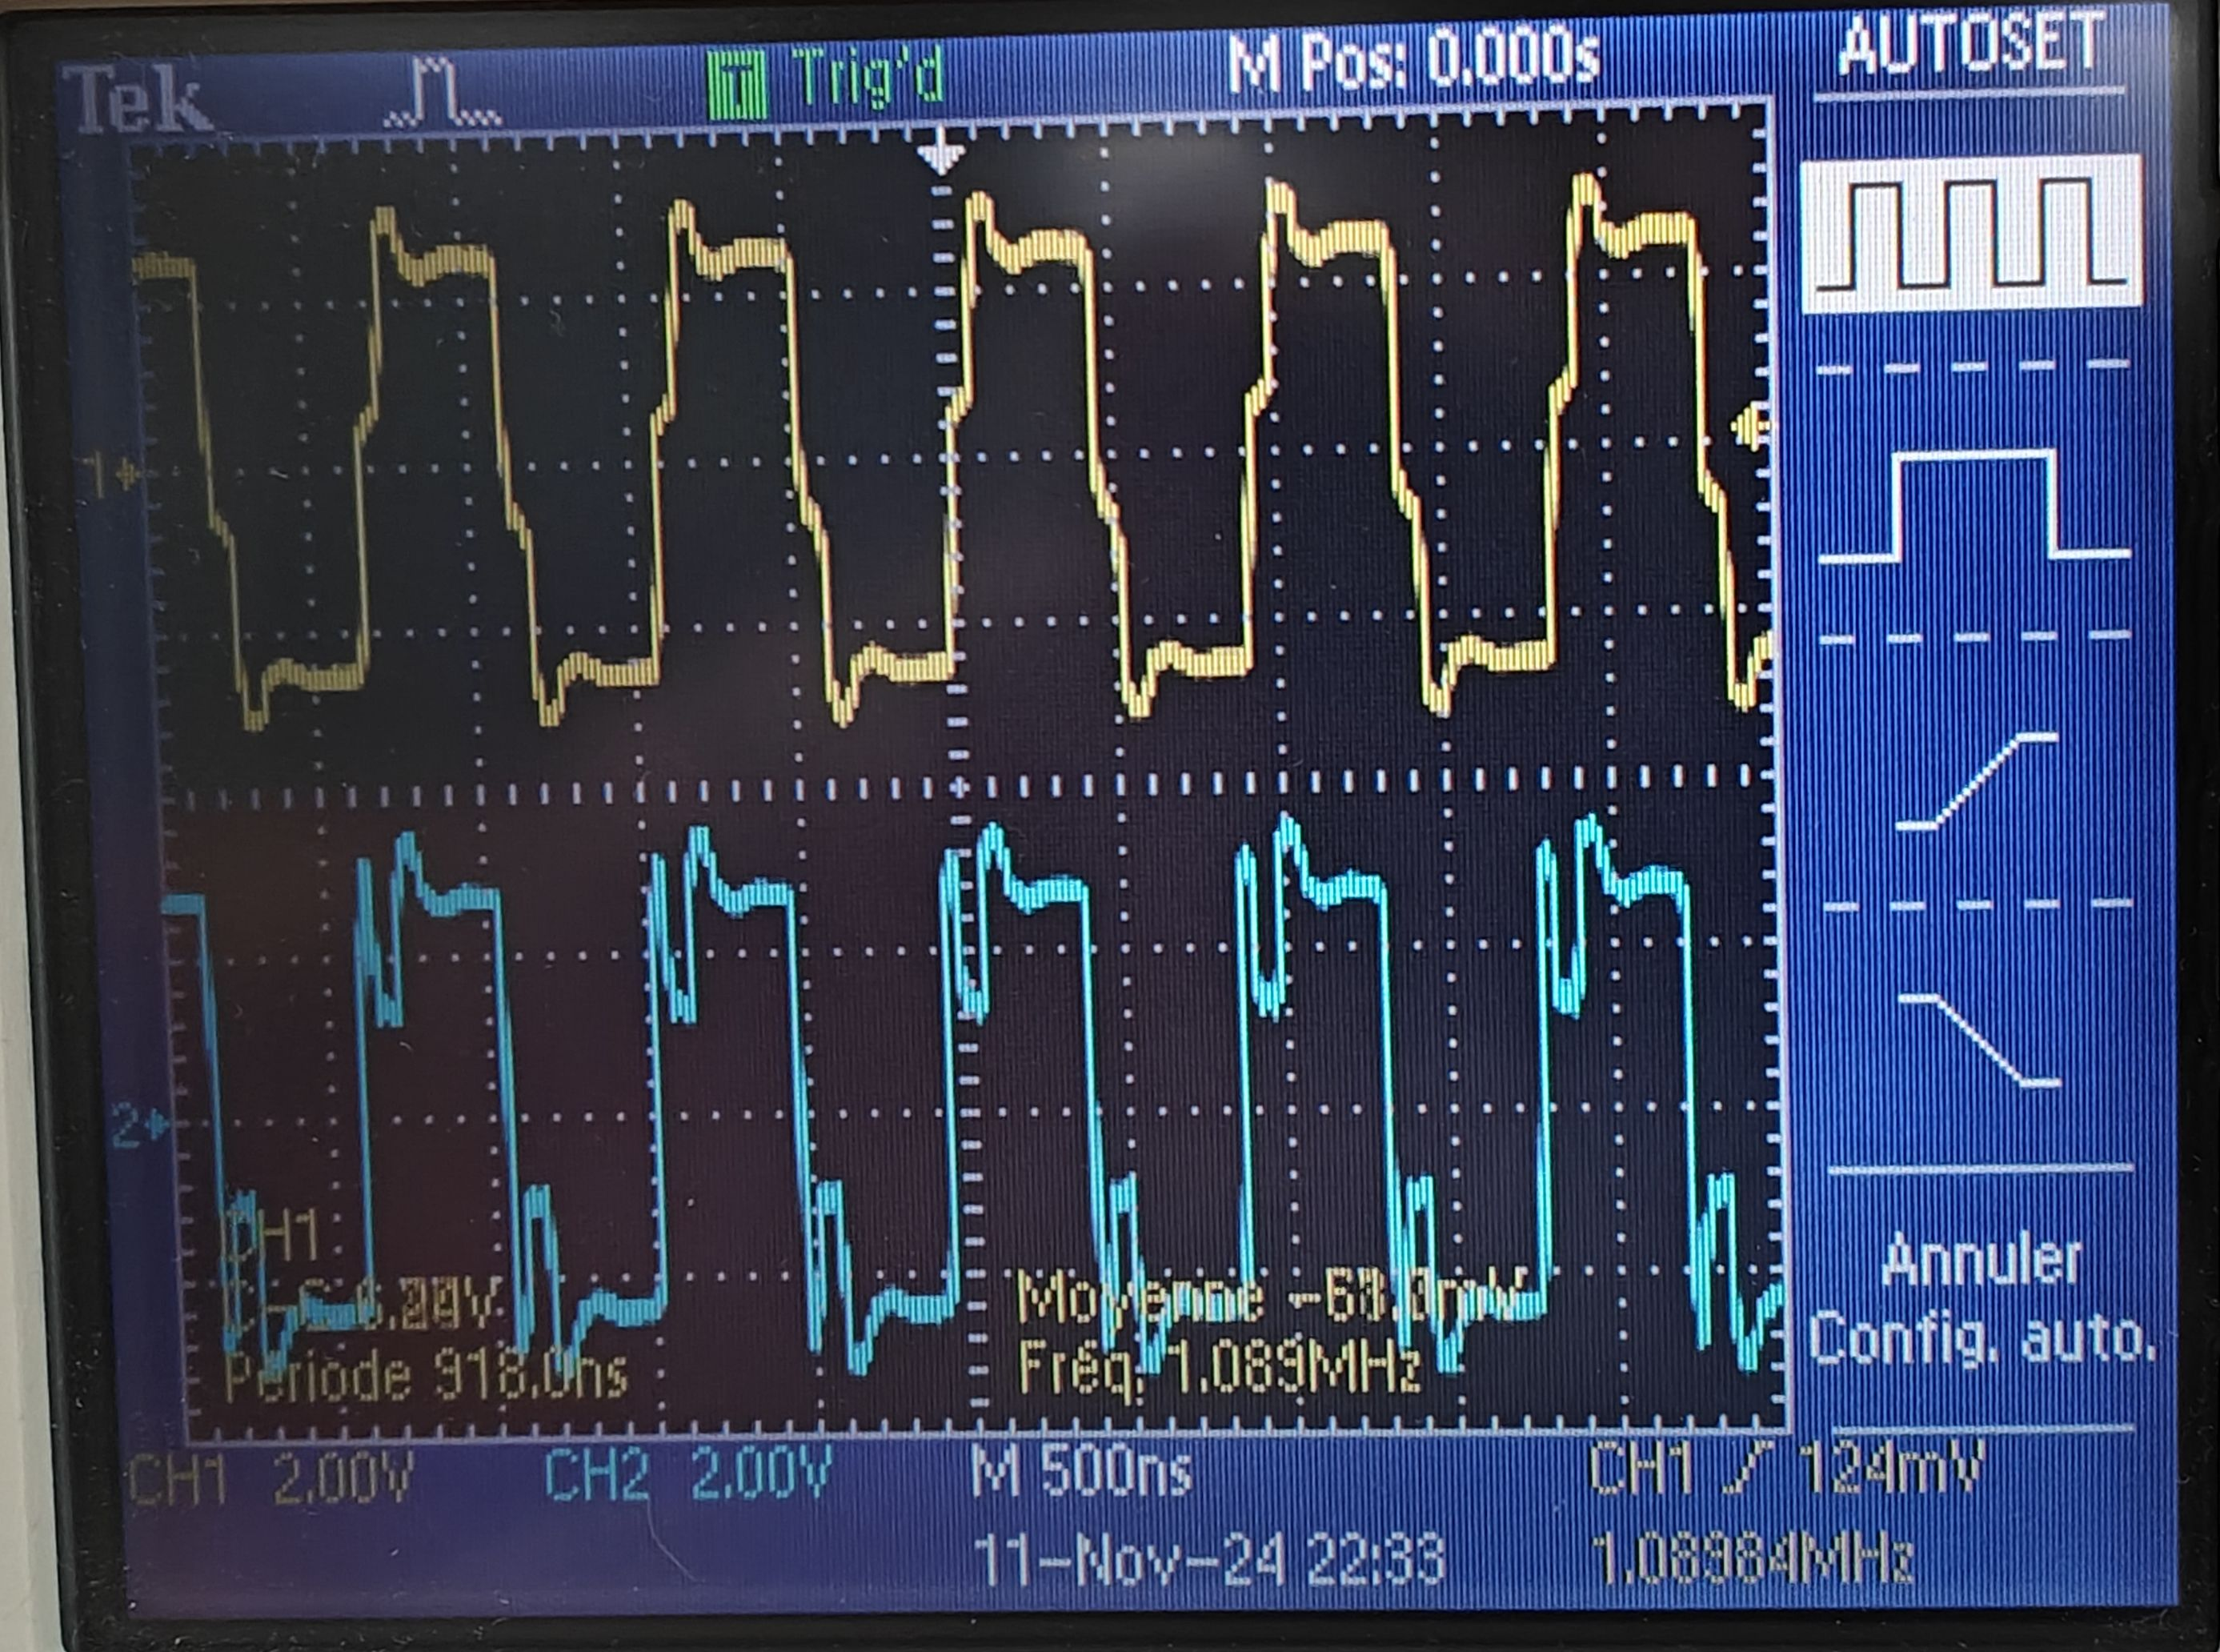
\includegraphics[width=0.7\textwidth]{images/1mhz.jpg}
    \caption{Diagramme de déploiement}
    \label{fig:Signal à 1MHz}
\end{figure}

Lorsque l'on observe le cycle de la ligne bleu, on peut voir que juste après le début de l'émission du signal, une descente se produit lorsque
la réflection du signal se produit et revient à l'entrée du circuit. La réflexion est aussi forte car lorsqu'un fil est laissé en circuit ouvert,
le coefficient de réflection est de 1. On peut observer que la ligne jaune ne semble pas avoir les mêmes "corrections" induites par la réflection
que la ligne bleu. Cela s'explique par le fait que la réflection a l'effet inverse sur la sortie. Si l'on observe attentivement, là où l'onde est
augmenté sur la ligne bleu, elle diminue sur la ligne jaune et vice-versa, mais à une amplitude réduite aussi.